
\documentclass[a4paper, 10pt, conference]{IEEEconf}  


%\usepackage{geometry}
%\geometry{a4paper, margin=1in}

    
\usepackage{verbatim}
\usepackage{graphicx}
\usepackage{pdfpages}
\usepackage{cite}



\setlength{\parskip}{1em}


\title{\LARGE \bf
Literature Review\\Prosthetic Tactile Sensor With Force Feedback
}

\author{Marc Alexander Sferrazza%
\thanks{*This work was not supported by any organization}%
\thanks{Faculty of Mechatronics Engineering, Massey University, Albany, Auckland, New Zealand
        {\tt\small Progress of project: alex1v1a.github.io /Prosthetic-Tactile-Research/}}%
}


\begin{document}

\begin{figure}
	\centering
	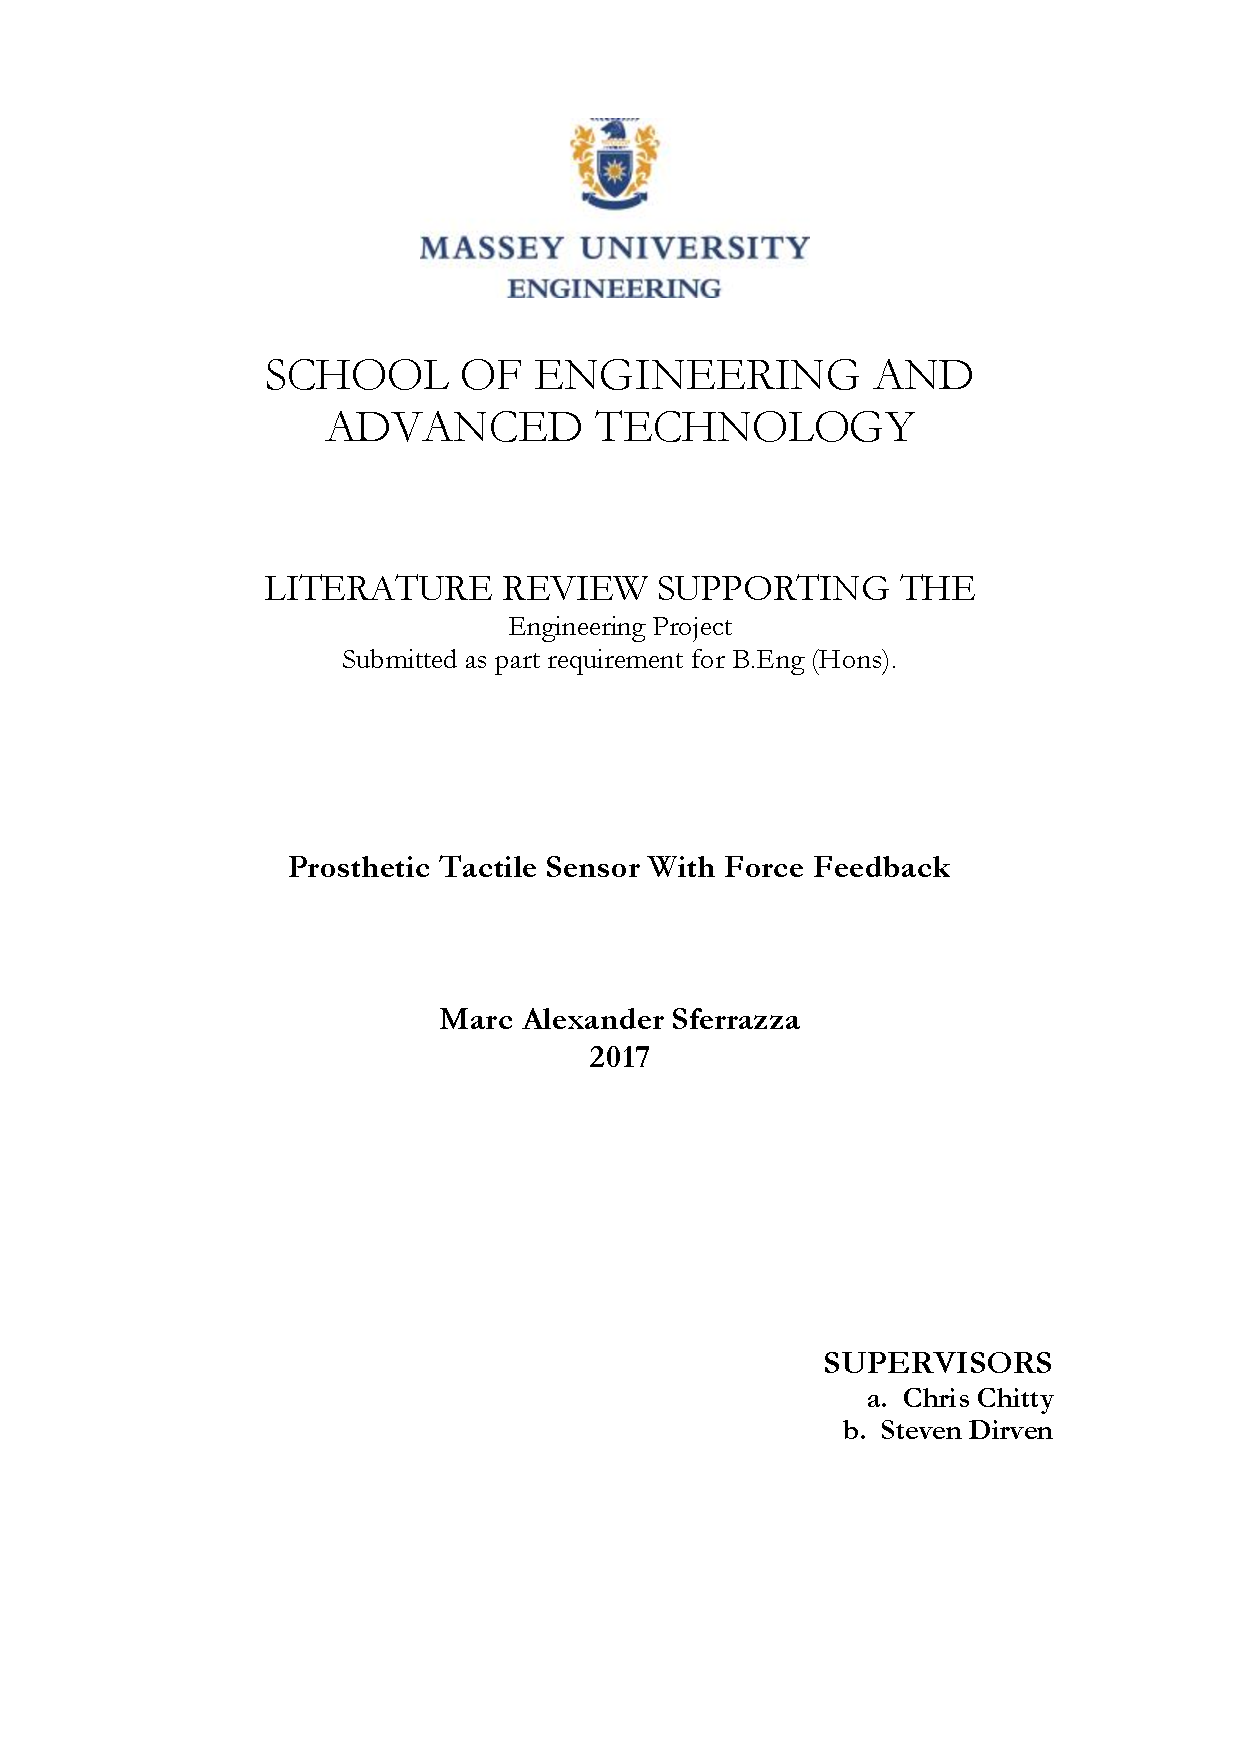
\includepdf[pages=-]{TitlePage.pdf}
\end{figure}

\

\maketitle
\thispagestyle{empty}
\pagestyle{empty}


\begin{abstract}



\end{abstract}


\section{INTRODUCTION}

\subsection{blah}

\begin{comment}
?	A concise definition of a topic under consideration (this may be a descriptive or agumentative thesis, or proposal), as well as the scope of the related literature being investigated. (Example: If the topic under consideration is `women's wartime diaries', the scope of the review may be limited to published or unpublished works, works in English, works from a particular location, time period, or conflict, etc.)
?	The introduction should also note intentional exclusions. (Example: "This review will not explore the diaries of adolescent girls.")
?	Another purpose of the introduction is to state the general findings of the review (what do most of the sources conclude), and comment on the availability of sources in the subject area.

Introductory section
o Explain why the review is carried out
o Describe the scope of the review
o Explain how the information in the
\end{comment}

\clearpage
\section{Review of Literature}

\subsection{blah}

\begin{comment}
?	There are many ways to organise the evaluation of the sources. Chronological and thematic approaches are each useful examples.
?	Each work should be critically summarised and evaluated for its premise, methodology, and conclusion. It is as important to address inconsistencies, omissions, and errors, as it is to identify accuracy, depth, and relevance.
?	Use logical connections and transitions to connect sources.

Relevant and logical flow of information
o Identify and discuss key areas of the research topic o Use of recent and relevant peer-reviewed journal
articles, books and other relevant material (e.g. reports
from previous work)
o Discuss techniques and equipment that are appropriate
for the research topic
o Identify gaps in the research
\end{comment}

\clearpage
\section{Methodology}

\subsection{blah}

\begin{comment}
this part here does this and this and this, this other part does this and this but we want to achieve this and this so we have chosen this sensor.

these sensors won?t work because of this and these sensors are ok for this but here are the faults

find where the research leads to and present it in that way for the end product and explaining things.

This is what the guy was explaining and not pulling things out of the sky.

Critical analysis
o Evaluate relevant research done by other researchers by ? Determining strengths and weaknesses of methods,
results, conclusions and recommendations ? Expressing and justifying agreement and
disagreement
\end{comment}




\begin{itemize}
	\item Be thorough and inclusive of all details concerning the decision 
	\item Be objective and not subjective to details central to the project
	\item Be aware of what the decision means or the outcome of the project
\end{itemize}	

\begin{comment}
\begin{figure}[h!]
  \includegraphics[width=\linewidth]{images/Timeline}
  \caption{Timeline}
  \label{fig:Timeline}
\end{figure}
\end{comment}

\clearpage
\section{CONCLUSIONS}

\begin{comment}
?	The conclusion summarizes the key findings of the review in general terms. Notable conunonalities between works, whether favourable or not, may be included here.
?	This section is the reviewer's opportunity to justify a research proposal. Therefore, the idea should be clearly re-stated and supported according to the findings of the review.
\end{comment}


\addtolength{\textheight}{-12cm}   % This command serves to balance the column lengths


\clearpage
\section*{APPENDIX}

\begin{comment}
?	As well as accurate in-text citations, a literature review must contain complete and correct citations for every source.

Referencing
o No plagiarism (all borrowed material must be adequately referenced).
o Consistent use of citation style throughout the chapter o Complete reference list

\end{comment}

\section*{ACKNOWLEDGMENT}


\nocite{*}
\bibliographystyle{ieeetr}
\bibliography{references}

\end{document}
